\documentclass[11pt,a4paper]{article}

\usepackage[a4paper,margin=2.54cm]{geometry}
\usepackage{setspace}
\usepackage{titlesec}
\usepackage{booktabs}
\usepackage{array}
\usepackage{graphicx}   % remove [draft] after uploading chart images to Overleaf
\usepackage{hyperref}
\usepackage{xcolor}
\usepackage{fancyhdr}
\usepackage{parskip}
\usepackage{amsmath}
\usepackage{float}
\usepackage{colortbl}
\usepackage{microtype}
\usepackage{enumitem}
\usepackage{helvet}           % Arial equivalent
\renewcommand{\familydefault}{\sfdefault}

\definecolor{regengreen}{RGB}{30,132,73}
\definecolor{darkgrey}{RGB}{26,26,26}
\definecolor{midgrey}{RGB}{85,85,85}
\definecolor{majorred}{RGB}{185,28,28}
\definecolor{moderateyellow}{RGB}{180,120,0}
\definecolor{tblhead}{RGB}{30,132,73}
\definecolor{tblalt}{RGB}{245,245,245}
\definecolor{placeholder}{RGB}{153,119,0}

\hypersetup{colorlinks=true,linkcolor=regengreen,citecolor=regengreen,urlcolor=regengreen}

\titleformat{\section}{\large\bfseries\color{darkgrey}}{\thesection.}{0.6em}{}[\titlerule]
\titleformat{\subsection}{\normalsize\bfseries\color{darkgrey}}{\thesubsection.}{0.5em}{}
\titleformat{\subsubsection}{\normalsize\itshape\color{darkgrey}}{\thesubsubsection.}{0.5em}{}

\pagestyle{fancy}
\fancyhf{}
\fancyhead[L]{\small\textit{300,000 Streets of Melbourne}}
\fancyhead[R]{\small\textit{School Streets Safety Analysis — Final Report}}
\fancyfoot[C]{\thepage}
\renewcommand{\headrulewidth}{0.4pt}

\setstretch{1.15}            % 1.15 line spacing

\newcolumntype{L}[1]{>{\raggedright\arraybackslash}p{#1}}
\newcolumntype{C}[1]{>{\centering\arraybackslash}p{#1}}

\graphicspath{{../docs/data/charts/}}

\setlist[itemize]{itemsep=1pt,topsep=3pt}
\setlist[enumerate]{itemsep=1pt,topsep=3pt}

\begin{document}

%% ── COVER PAGE ────────────────────────────────────────────────
\begin{titlepage}
\centering\vspace*{1.2cm}
{\Large\bfseries\color{regengreen}300,000 Streets of Melbourne}\\[0.4cm]
{\LARGE\bfseries School Streets Safety Analysis}\\[0.3cm]
{\large\itshape Healthy Streets Assessment for Secondary School Walking Routes, Darebin, Victoria}
\vspace{1cm}

\rule{0.6\textwidth}{1.5pt}\\[0.8cm]
{\large\bfseries Final Project Report}\\[0.3cm]
{\normalsize COSC2667 / COSC2777 — Data Science and AI Postgraduate Projects}
\vspace{1.2cm}

{\normalsize\begin{tabular}{rl}
\textbf{Industry Partner:}       & Regen Melbourne \\[0.3em]
\textbf{Industrial Supervisor:}  & Nina Sharpe \\[0.3em]
\textbf{Academic Supervisor:}    & Lawrence Cavedon \\[0.3em]
\textbf{Student Team:}           & Hishikesh Phukan (S4031214) \\
                                 & Reddy Pranay Vipparla (S4112678) \\
                                 & Venkata Nagendra Anamala (S4024233) \\
                                 & Siddhartha Ananthula (S4111078) \\
                                 & Sameer Yadav (S4038689) \\[0.3em]
\textbf{Date:}                   & June 2026 \\
\end{tabular}}
\vfill
{\small\itshape Data: data.vic.gov.au $\cdot$ OpenStreetMap $\cdot$ EPA Victoria $\cdot$ ABS 2021 $\cdot$ CSA Victoria}
\end{titlepage}

%% ── 1. INTRODUCTION ──────────────────────────────────────────
\section{Introduction}

\subsection{Partner Organisation — Regen Melbourne}
Regen Melbourne is a not-for-profit urban regeneration organisation focused on transforming Melbourne's streets from car-dominated corridors into safe, liveable, and community-centred spaces. Their \textit{300,000 Streets of Melbourne} initiative aims to retrofit the street network to prioritise walking, cycling, and public life. Regen Melbourne's 300,000 Streets initiative ultimately seeks to assess and improve street conditions around schools across Greater Melbourne, a network of over 300 secondary schools spanning hundreds of suburbs. However, conducting field observations and detailed spatial analysis at this scale within a ten-week academic project was not feasible. In consultation with the industry partner, the project team scoped the study to three secondary schools in the City of Darebin (Reservoir High School, William Ruthven Secondary College, and Preston High School) as a representative pilot. These schools were selected because Darebin combines arterial road pressure, socio-economic diversity, and dense active-travel demand, making it an informative test case for a methodology intended to scale. The pipeline, scoring model, and dashboard developed here are explicitly designed to be replicated across additional schools with no changes to the codebase.

The assessment methodology underpinning this project is the \textbf{Healthy Streets framework}, developed by Lucy Saunders for Transport for London (Saunders, 2015). The framework defines ten human-centred indicators (HS1--HS10) spanning pedestrian priority, road crossing safety, shade and shelter, rest amenity, noise, active travel infrastructure, perceived safety, destination diversity, environmental quality, and air quality. Each indicator is scored 0--10 and a composite index is derived by averaging across all ten, providing a structured, replicable, and evidence-based tool for assessing the walkability of street environments around schools. The Healthy Streets framework was chosen because it is widely adopted by transport authorities in the United Kingdom and Australasia, aligns directly with Regen Melbourne's street improvement agenda, and is designed to be applied by non-specialist assessors using a combination of field observation and open data.

\subsection{Project Aims}

\textbf{Initial aims (as per project proposal):}
\begin{itemize}
  \item Assess pedestrian and cycling safety for walking routes around three Darebin secondary schools using the Healthy Streets framework (Saunders, 2015).
  \item Produce quantified scores and prioritised intervention recommendations per school.
  \item Deliver outputs accessible to Regen Melbourne's non-technical stakeholders.
\end{itemize}

\textbf{Current aims (expanded during delivery):}
\begin{itemize}
  \item All initial aims, plus:
  \item Train a machine learning model to predict HS indicator scores from open data, enabling network-wide screening of Melbourne's 200+ secondary schools without field surveys.
  \item Build a what-if scenario engine modelling the predicted impact of ten physical interventions per school.
  \item Conduct an equity analysis linking socioeconomic disadvantage (ABS SEIFA 2021) to safety outcomes.
  \item Analyse Victorian road crash trends (2021--2025) near school gates.
  \item Deploy all findings as an interactive GitHub Pages dashboard.
\end{itemize}

The scope expanded because Regen Melbourne expressed interest in a \textit{scalable} methodology for the broader Melbourne school network, and the equity finding (more disadvantaged catchments have worse safety outcomes) emerged as an important and unplanned policy insight during data exploration.

\subsection{Study Area — School Profiles}

The three pilot schools are located within the City of Darebin, an inner-northern Melbourne local government area characterised by a mix of arterial roads, tram corridors, and residential streets with varying footpath quality. Table~1 summarises the key characteristics of each school.

\begin{table}[H]\centering\small
\caption{School profiles — City of Darebin pilot study}
\begin{tabular}{L{3.2cm}L{3.5cm}L{1.5cm}L{2cm}L{3.8cm}}
\toprule
\textbf{School} & \textbf{Address} & \textbf{Type} & \textbf{SEIFA Decile} & \textbf{Key hazard context} \\
\midrule
Reservoir High School & 855 Plenty Rd, Reservoir VIC 3073r & Gov. secondary & 4 & Fronts Plenty Road arterial; limited crossing infrastructure \\
William Ruthven SC & 60 Merrilands Rd, Reservoir VIC 3073 & Gov. secondary & 6 & Inner-suburban; poor shade/rest amenity \\
Preston High School &  2-16 Cooma St, Preston VIC 3072 & Gov. secondary & 7 & No signalised crossing at gate; HS2 = 0.4 \\
\bottomrule
\end{tabular}
\end{table}

\subsection{Deliverables}

\begin{table}[H]\centering\small
\begin{tabular}{C{0.6cm}L{3cm}L{10cm}}
\toprule
\textbf{ID} & \textbf{Deliverable} & \textbf{Description} \\
\midrule
D1 & HS assessment & Quantified HS1--HS10 scores, hazard severity, and recommendations for 3 schools \\
D2 & ML prediction model & Trained Ridge regression model predicting HS scores from open data \\
D3 & Scenario engine & 10 intervention templates with delta-method impact prediction \\
D4 & Equity analysis & SEIFA--safety correlation with supporting visualisations \\
D5 & Crash trend analysis & VicRoads crash data (2021--2025) with school-hours breakdown \\
D6 & Interactive dashboard & GitHub Pages dashboard (7 sections, layer-enabled map, scenario explorer) \\
D7 & This report & Final project report per COSC2667/2777 guidelines \\
\bottomrule
\end{tabular}
\end{table}

%% ── 2. METHODOLOGY ───────────────────────────────────────────
\section{Methodology}

\subsection{Overall Approach}
The project follows a ten-step reproducible pipeline that transforms raw field observations and open government data into scored assessments, ML predictions, equity analysis, crash trends, scenario modelling, and a stakeholder dashboard. Each pipeline step links to a project aim: steps 1--4 deliver D1 (assessment), steps 5--6 deliver D2 (ML), steps 7--8 deliver D4 (equity), step 9 delivers D5 (crashes), and the dashboard pipeline delivers D6.

\begin{figure}[H]\centering

\includegraphics[width=0.93\textwidth]{chart1_safety_scores.png}
\caption{Figure 1 — Healthy Streets indicator scores across all three assessed schools}
\end{figure}

\subsection{Healthy Streets Framework and Scoring (D1)}
Each school gate is scored across ten indicators (HS1--HS10, scored 0--10). Five indicators (HS1, HS2, HS5, HS7, HS9) are scored from field observation; five (HS3, HS4, HS6, HS8, HS10) from open data. Overall score = mean across all indicators. Severity: \textbf{Major} (HS2$<$4.0 or HS1$<$4.0 or HS5$<$3.0), \textbf{Moderate} (2+ indicators $<$6.0 or overall$<$5.0), \textbf{Minor} (otherwise). A rule engine (17 rules tagged to HS indicators) generates prioritised recommendations. Table~2 defines each indicator and its data source.

\begin{table}[H]\centering\small
\caption{Healthy Streets indicators — definitions and scoring basis}
\setlength{\tabcolsep}{4pt}
\begin{tabular}{C{0.7cm}L{3cm}L{5.5cm}L{4.8cm}}
\toprule
\textbf{ID} & \textbf{Name} & \textbf{What it measures} & \textbf{Scoring basis} \\
\midrule
HS1 & Pedestrian priority & Footpath width, continuity, kerb ramps, surface condition & Field observation \\
HS2 & Easy to cross & Crossing type, proximity to gate, sight lines & Field observation \\
HS3 & Shade \& shelter & Tree canopy, bus shelters along route & OSM tree count / shelter count (400m) \\
HS4 & Places to rest & Bench density, seating availability & OSM bench count (400m) \\
HS5 & Not too noisy & Traffic volume, speed zone at gate & Field observation \\
HS6 & Active travel choice & Cycling infrastructure coverage, PT stop accessibility & OSM cycle path length + PT stops (400m) \\
HS7 & Feel safe & Perceived safety, crime rate & CSA crime rate (suburb-level) \\
HS8 & Things to do & Destination diversity, active frontages & OSM POI count (400m) \\
HS9 & Feel relaxed & Street litter, graffiti, environmental quality & Field observation \\
HS10 & Clean air & Ambient PM2.5 concentration & EPA AirWatch annual average \\
\bottomrule
\end{tabular}
\end{table}

\subsection{Data Sources and Justification}

\begin{table}[H]\centering\small
\begin{tabular}{L{3.2cm}L{4.2cm}L{1.8cm}L{4.3cm}}
\toprule
\textbf{Dataset} & \textbf{Source / URL} & \textbf{Volume} & \textbf{Used for} \\
\midrule
Field observation & RMIT / Regen Melbourne & 3 schools & HS1, HS2, HS5, HS7, HS9 \\
Victorian Road Crash Data & \href{https://www.data.vic.gov.au}{data.vic.gov.au} & 7,948 records & Crash analysis (D5) \\
OpenStreetMap (osmnx) & \href{https://www.openstreetmap.org}{openstreetmap.org} via Overpass API & 53 features/school & HS3, HS4, HS6, HS8, ML \\
EPA AirWatch PM2.5 & \href{https://www.epa.vic.gov.au/for-community/monitoring-the-environment/airwatch}{epa.vic.gov.au/airwatch} & Annual average & HS10 \\
Crime rate & \href{https://www.crimestatistics.vic.gov.au}{crimestatistics.vic.gov.au} & Suburb-level & HS7 \\
ABS SEIFA 2021 IRSD & \href{https://www.abs.gov.au/statistics/people/people-and-communities/socio-economic-indexes-areas-seifa-australia/2021}{abs.gov.au/seifa-2021} & 3 catchments & Equity analysis (D4) \\
ABS Census 2021 & \href{https://www.abs.gov.au/census}{abs.gov.au/census} & Suburb level & Demographics \\
\bottomrule
\end{tabular}
\end{table}

OSM was chosen as the primary spatial data source because it is freely available, programmatically accessible via \texttt{osmnx}, and covers walking networks, cycling infrastructure, amenity, and crossings at 200m/400m/800m radii. All spatial operations use EPSG:7855 (GDA2020 / MGA zone 55), the Victorian standard for metric accuracy.

\subsection{Machine Learning — HS Score Prediction (D2)}

\textbf{Aim:} can open-data features predict HS scores reliably enough to replace or reduce field surveys when scaling to 200+ schools?

\textbf{Feature matrix:} 26 open-data features (20 OSM spatial, 2 environmental, 4 crash aggregates). Target: HS1--HS10 per school.

\textbf{Model choice (Ridge regression):} With only $n=3$ schools, regularisation is essential. Ridge (L2 penalty) shrinks coefficients without zeroing them, which is appropriate for feature-rich, small-sample settings. Random Forest was considered but rejected because it memorises $n=3$ training points (zero training error, no generalisation). Lasso was tested but produced overly sparse solutions at this sample size.

\textbf{Evaluation (LOO-CV):} A standard train/test split is meaningless with $n=3$. Leave-One-Out CV produces 3 independent predictions and computes MAE per indicator.

\textbf{Baseline:} Predicting the sample mean for all schools gives MAE $\approx 2.1$ averaged across indicators.

\subsection{What-If Scenario Engine (D3)}
The delta method models physical interventions without retraining:
\[\text{score}_\text{scenario}[i] = \text{score}_\text{actual}[i] + \bigl(\hat{f}(X_\text{scenario})[i] - \hat{f}(X_\text{baseline})[i]\bigr)\]
This eliminates model bias by anchoring to actual scores and using the model only to estimate the change. Ten templates define which OSM features change; all 30 results (10$\times$3) are pre-computed and embedded in \texttt{data.json} for instant browser rendering.

\subsection{Computational Environment}

\begin{table}[H]\centering\small
\begin{tabular}{L{3.5cm}L{10cm}}
\toprule
\textbf{Component} & \textbf{Specification} \\
\midrule
Language & Python 3.10+ \\
Key libraries & pandas, numpy, geopandas, osmnx, scikit-learn, matplotlib, folium \\
ML framework & scikit-learn: MultiOutputRegressor(Ridge($\alpha$=1.0)) + StandardScaler \\
CRS / GIS & EPSG:7855 (GDA2020 / MGA zone 55) via pyogrio / geopandas \\
Dashboard & Static HTML/JS — Chart.js 4, Leaflet 1.9, Leaflet.heat, Tailwind CSS \\
Hosting & GitHub Pages (static; all 30 scenarios pre-computed at build time) \\
Repository & github.com/s4111078-sidd/300-000-School-Streets \\
\bottomrule
\end{tabular}
\end{table}

%% ── 3. RESULTS, EVALUATION & ANALYSIS ───────────────────────
\newpage
\section{Results, Evaluation \& Analysis}

\subsection{D1 — Healthy Streets Assessment}

\begin{table}[H]\centering\small
\caption{Healthy Streets Indicator Scores}
\setlength{\tabcolsep}{4pt}
\begin{tabular}{L{2.8cm}C{0.5cm}C{0.5cm}C{0.5cm}C{0.5cm}C{0.5cm}C{0.5cm}C{0.5cm}C{0.5cm}C{0.5cm}C{0.6cm}C{0.85cm}C{1.5cm}}
\toprule
\textbf{School} & \textbf{1} & \textbf{2} & \textbf{3} & \textbf{4} & \textbf{5} & \textbf{6} & \textbf{7} & \textbf{8} & \textbf{9} & \textbf{10} & \textbf{Overall} & \textbf{Severity} \\
\midrule
Reservoir HS & 4.2 & 5.7 & 5.0 & 6.0 & 5.0 & 6.0 & 8.0 & 6.8 & 5.2 & 9.0 & 6.1 & \textcolor{moderateyellow}{\textbf{Moderate}} \\
William Ruthven SC & 9.5 & 6.8 & 3.0 & 3.3 & 10.0 & 4.2 & 7.5 & 4.3 & 8.0 & 10.0 & 6.7 & \textcolor{moderateyellow}{\textbf{Moderate}} \\
Preston HS & 9.1 & \textcolor{majorred}{\textbf{0.4}} & 5.0 & 8.0 & 7.0 & 7.8 & 8.0 & 10.0 & 7.6 & 9.0 & 7.2 & \textcolor{majorred}{\textbf{Major}} \\
\midrule
\textit{Target} & \textit{6} & \textit{6} & \textit{6} & \textit{6} & \textit{6} & \textit{6} & \textit{6} & \textit{6} & \textit{6} & \textit{6} & \textit{6.0} & --- \\
\bottomrule
\end{tabular}
\end{table}

Preston HS is \textbf{Major} because HS2 = 0.4 — there is no formal crossing at the school gate on Cooma Street. Students must cross an unsignalised mid-block location, creating acute risk during the 08:00--09:00 and 15:00--16:00 peaks. Reservoir HS has five indicators below the 6.0 target (HS1, HS2, HS3, HS5, HS9), driven by its Plenty Road arterial frontage: high traffic volume suppresses pedestrian priority (HS1), crossing safety (HS2), noise (HS5), and perceived relaxation (HS9), while the exposed corridor has minimal tree canopy (HS3). William Ruthven SC scores Moderate despite a relatively lower-risk road environment, because critically low shade (HS3 = 3.0) and rest amenity (HS4 = 3.3) consistently fail the 6.0 threshold. All three schools score well on HS7 (feel safe, crime rate) and HS10 (clean air, PM2.5), reflecting Darebin's low crime rate and distance from industrial emission sources.

\subsection{D2 — ML Performance and Evaluation}

\begin{table}[H]\centering\small
\caption{LOO-CV MAE per Indicator vs.\ Baseline ($n=3$)}
\begin{tabular}{L{4cm}C{2cm}C{2.5cm}L{5.5cm}}
\toprule
\textbf{Indicator} & \textbf{Ridge MAE} & \textbf{Baseline MAE} & \textbf{Automatable?} \\
\midrule
HS7 — Feel safe & 0.54 & 1.8 & Yes — crime rate is reliable proxy \\
HS10 — Clean air & 0.92 & 0.9 & Yes — PM2.5 maps directly \\
HS9 — Feel relaxed & 1.72 & 1.7 & Largely \\
HS3 — Shade/shelter & 2.17 & 3.0 & Partial \\
HS1 — Pedestrians & 3.27 & 2.7 & Partial \\
HS5 — Not too noisy & 3.68 & 2.4 & Partial \\
HS4 — Rest places & 4.19 & 3.1 & No — OSM bench data sparse \\
HS2 — Easy to cross & 4.51 & 2.2 & No — quality $\neq$ presence \\
HS8 — Things to do & 4.72 & 2.9 & No — activity quality not in OSM \\
\midrule
\textbf{Mean} & \textbf{2.88} & \textbf{2.1} & --- \\
\bottomrule
\end{tabular}
\end{table}

HS7 substantially beats the baseline (MAE 0.54 vs 1.8); HS10 matches it (MAE 0.92 vs 0.9); both are practically automatable but for different reasons: crime rate is a strong proxy for perceived safety (HS7), while PM2.5 variance is simply very low across Darebin making any predictor appear accurate (HS10). HS2, HS4, and HS8 do not beat the baseline; field surveys remain necessary for these. A two-stage screening approach can automate HS7/HS10, partially automate HS3/HS6/HS9, and deploy field surveyors only for HS1/HS2/HS4/HS5/HS8 at flagged schools. Full component-level scoring rubrics and severity classification thresholds are provided in Appendix~D.

\begin{figure}[H]\centering
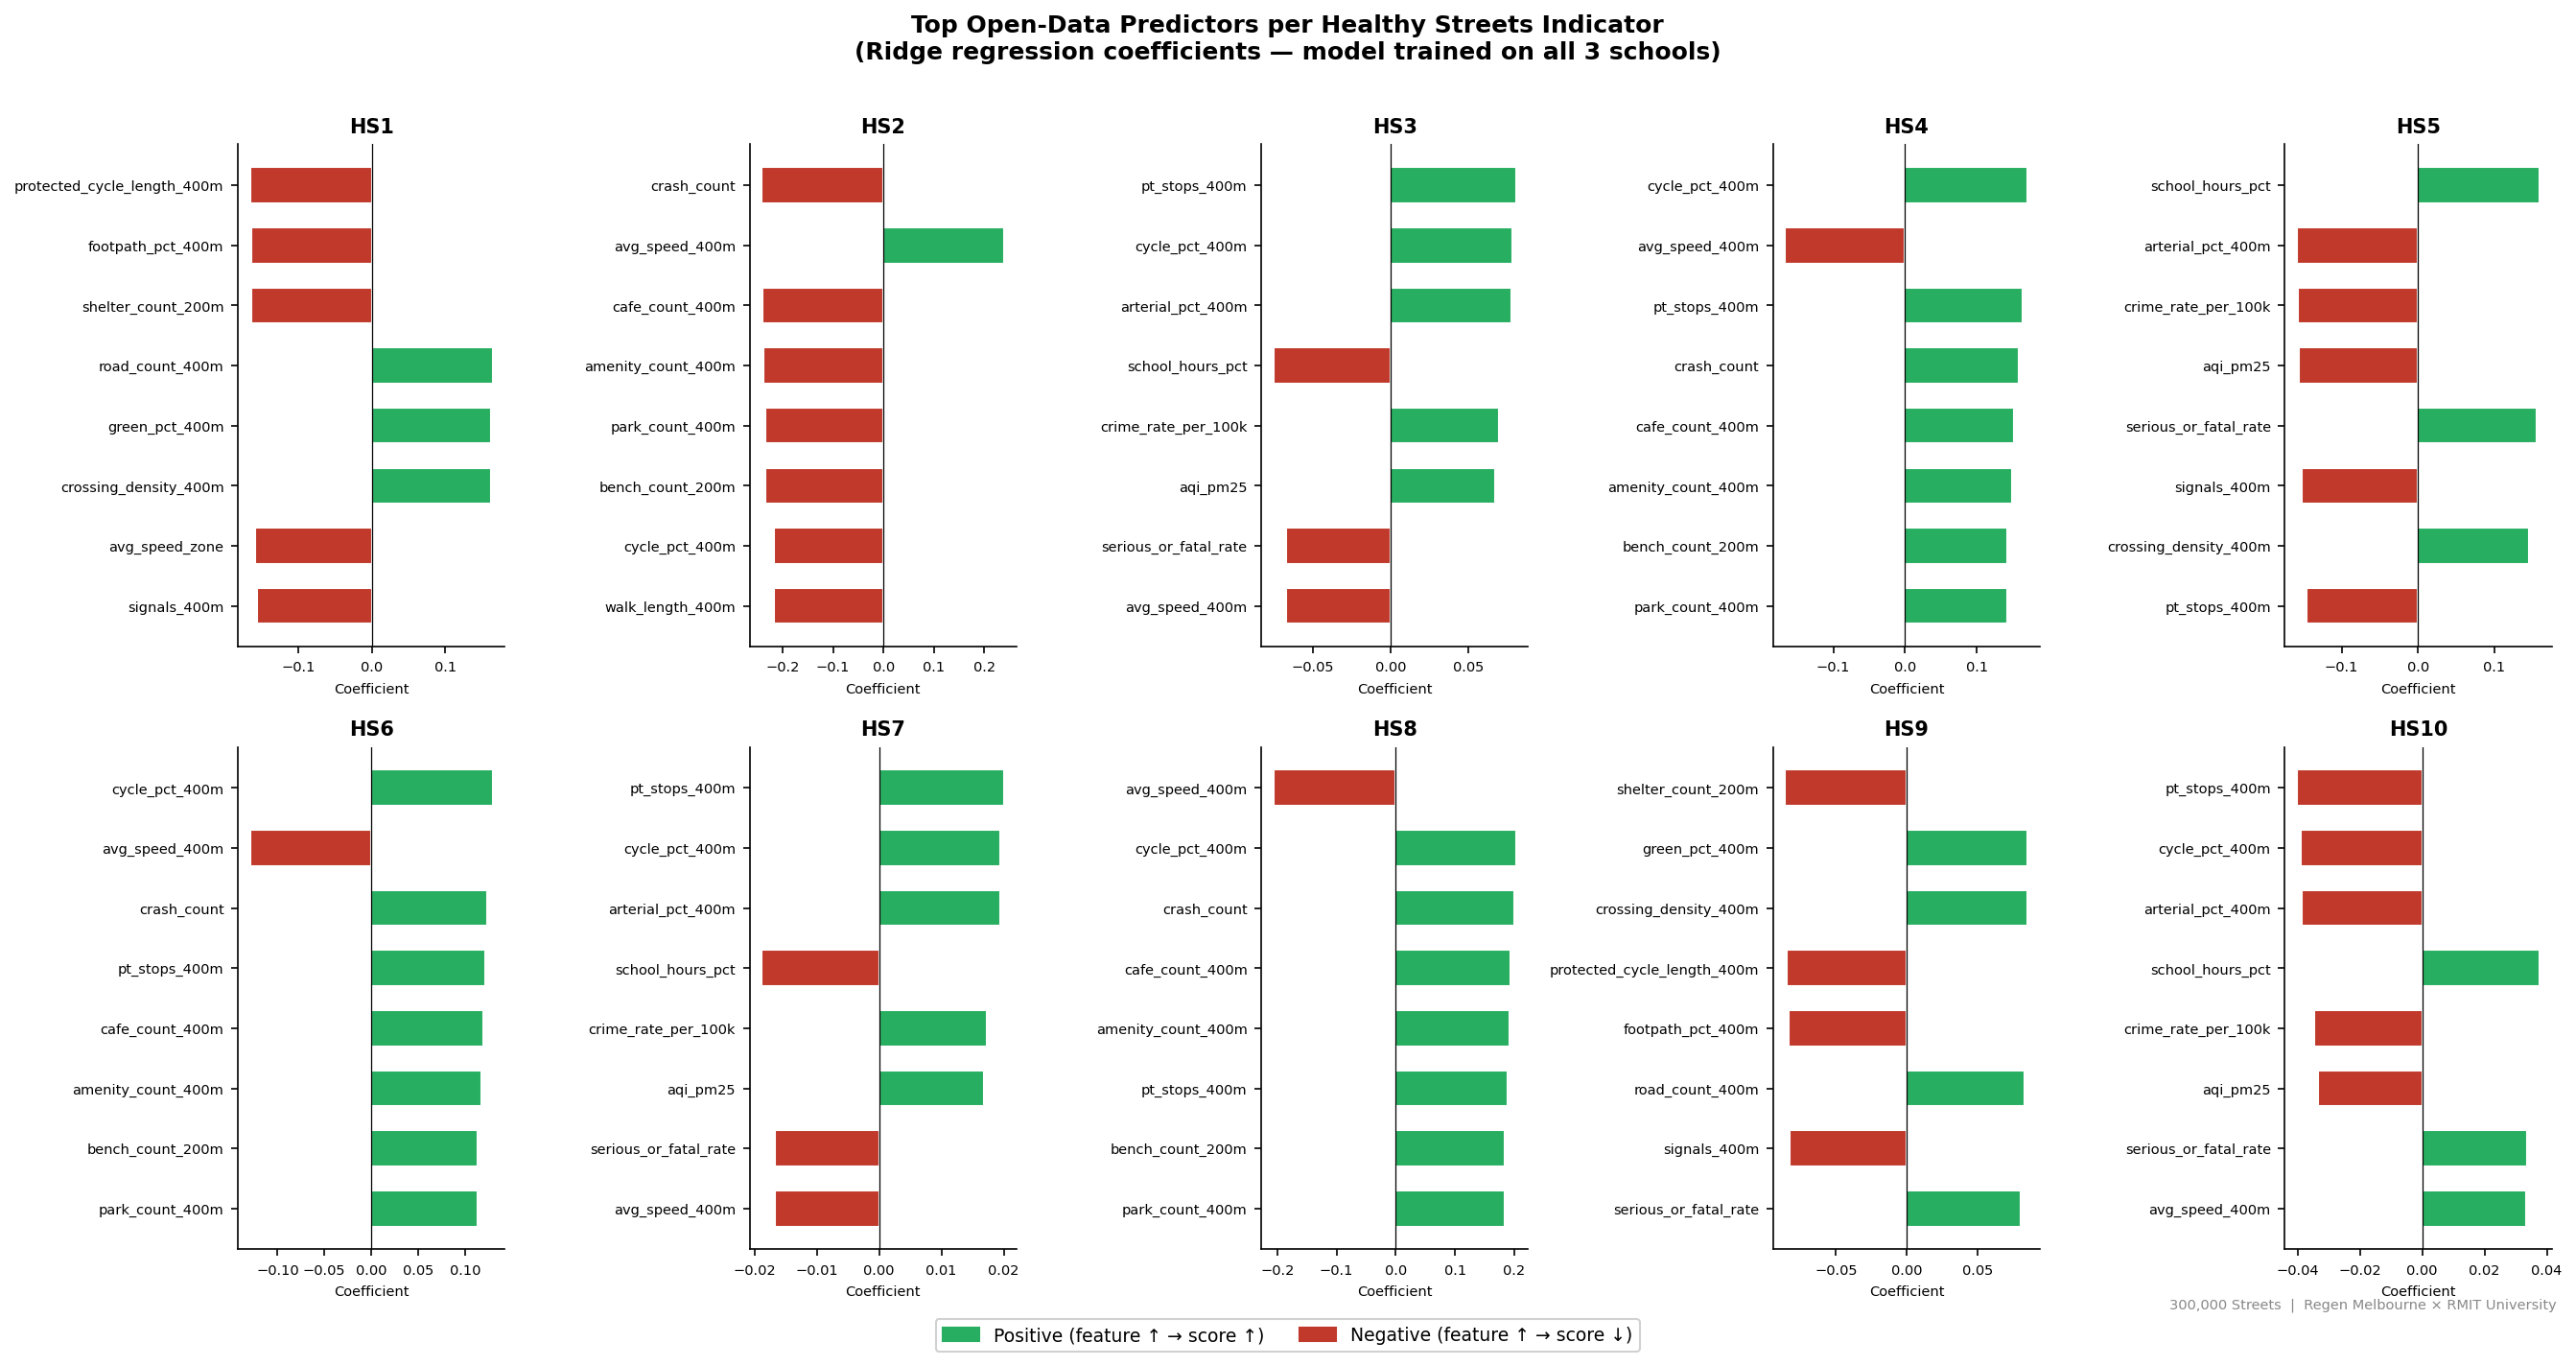
\includegraphics[width=0.93\textwidth]{chart_feature_importance.png}
\caption{Figure 2 — Ridge regression coefficients: top open-data predictors per HS indicator}
\end{figure}

\subsection{D4 — Equity Analysis}
Pearson $r = 0.84$ between SEIFA IRSD decile and overall HS score ($n=3$). More disadvantaged catchments have worse safety outcomes: Reservoir HS (Decile 4, national lower 40th percentile) has the lowest score (6.1) and most below-threshold indicators (five). This finding, consistent with Giles-Corti et al.\ (2016), supports equity-weighted investment criteria prioritising Reservoir HS, which satisfies both high risk and high disadvantage simultaneously.

\begin{figure}[htbp]\centering
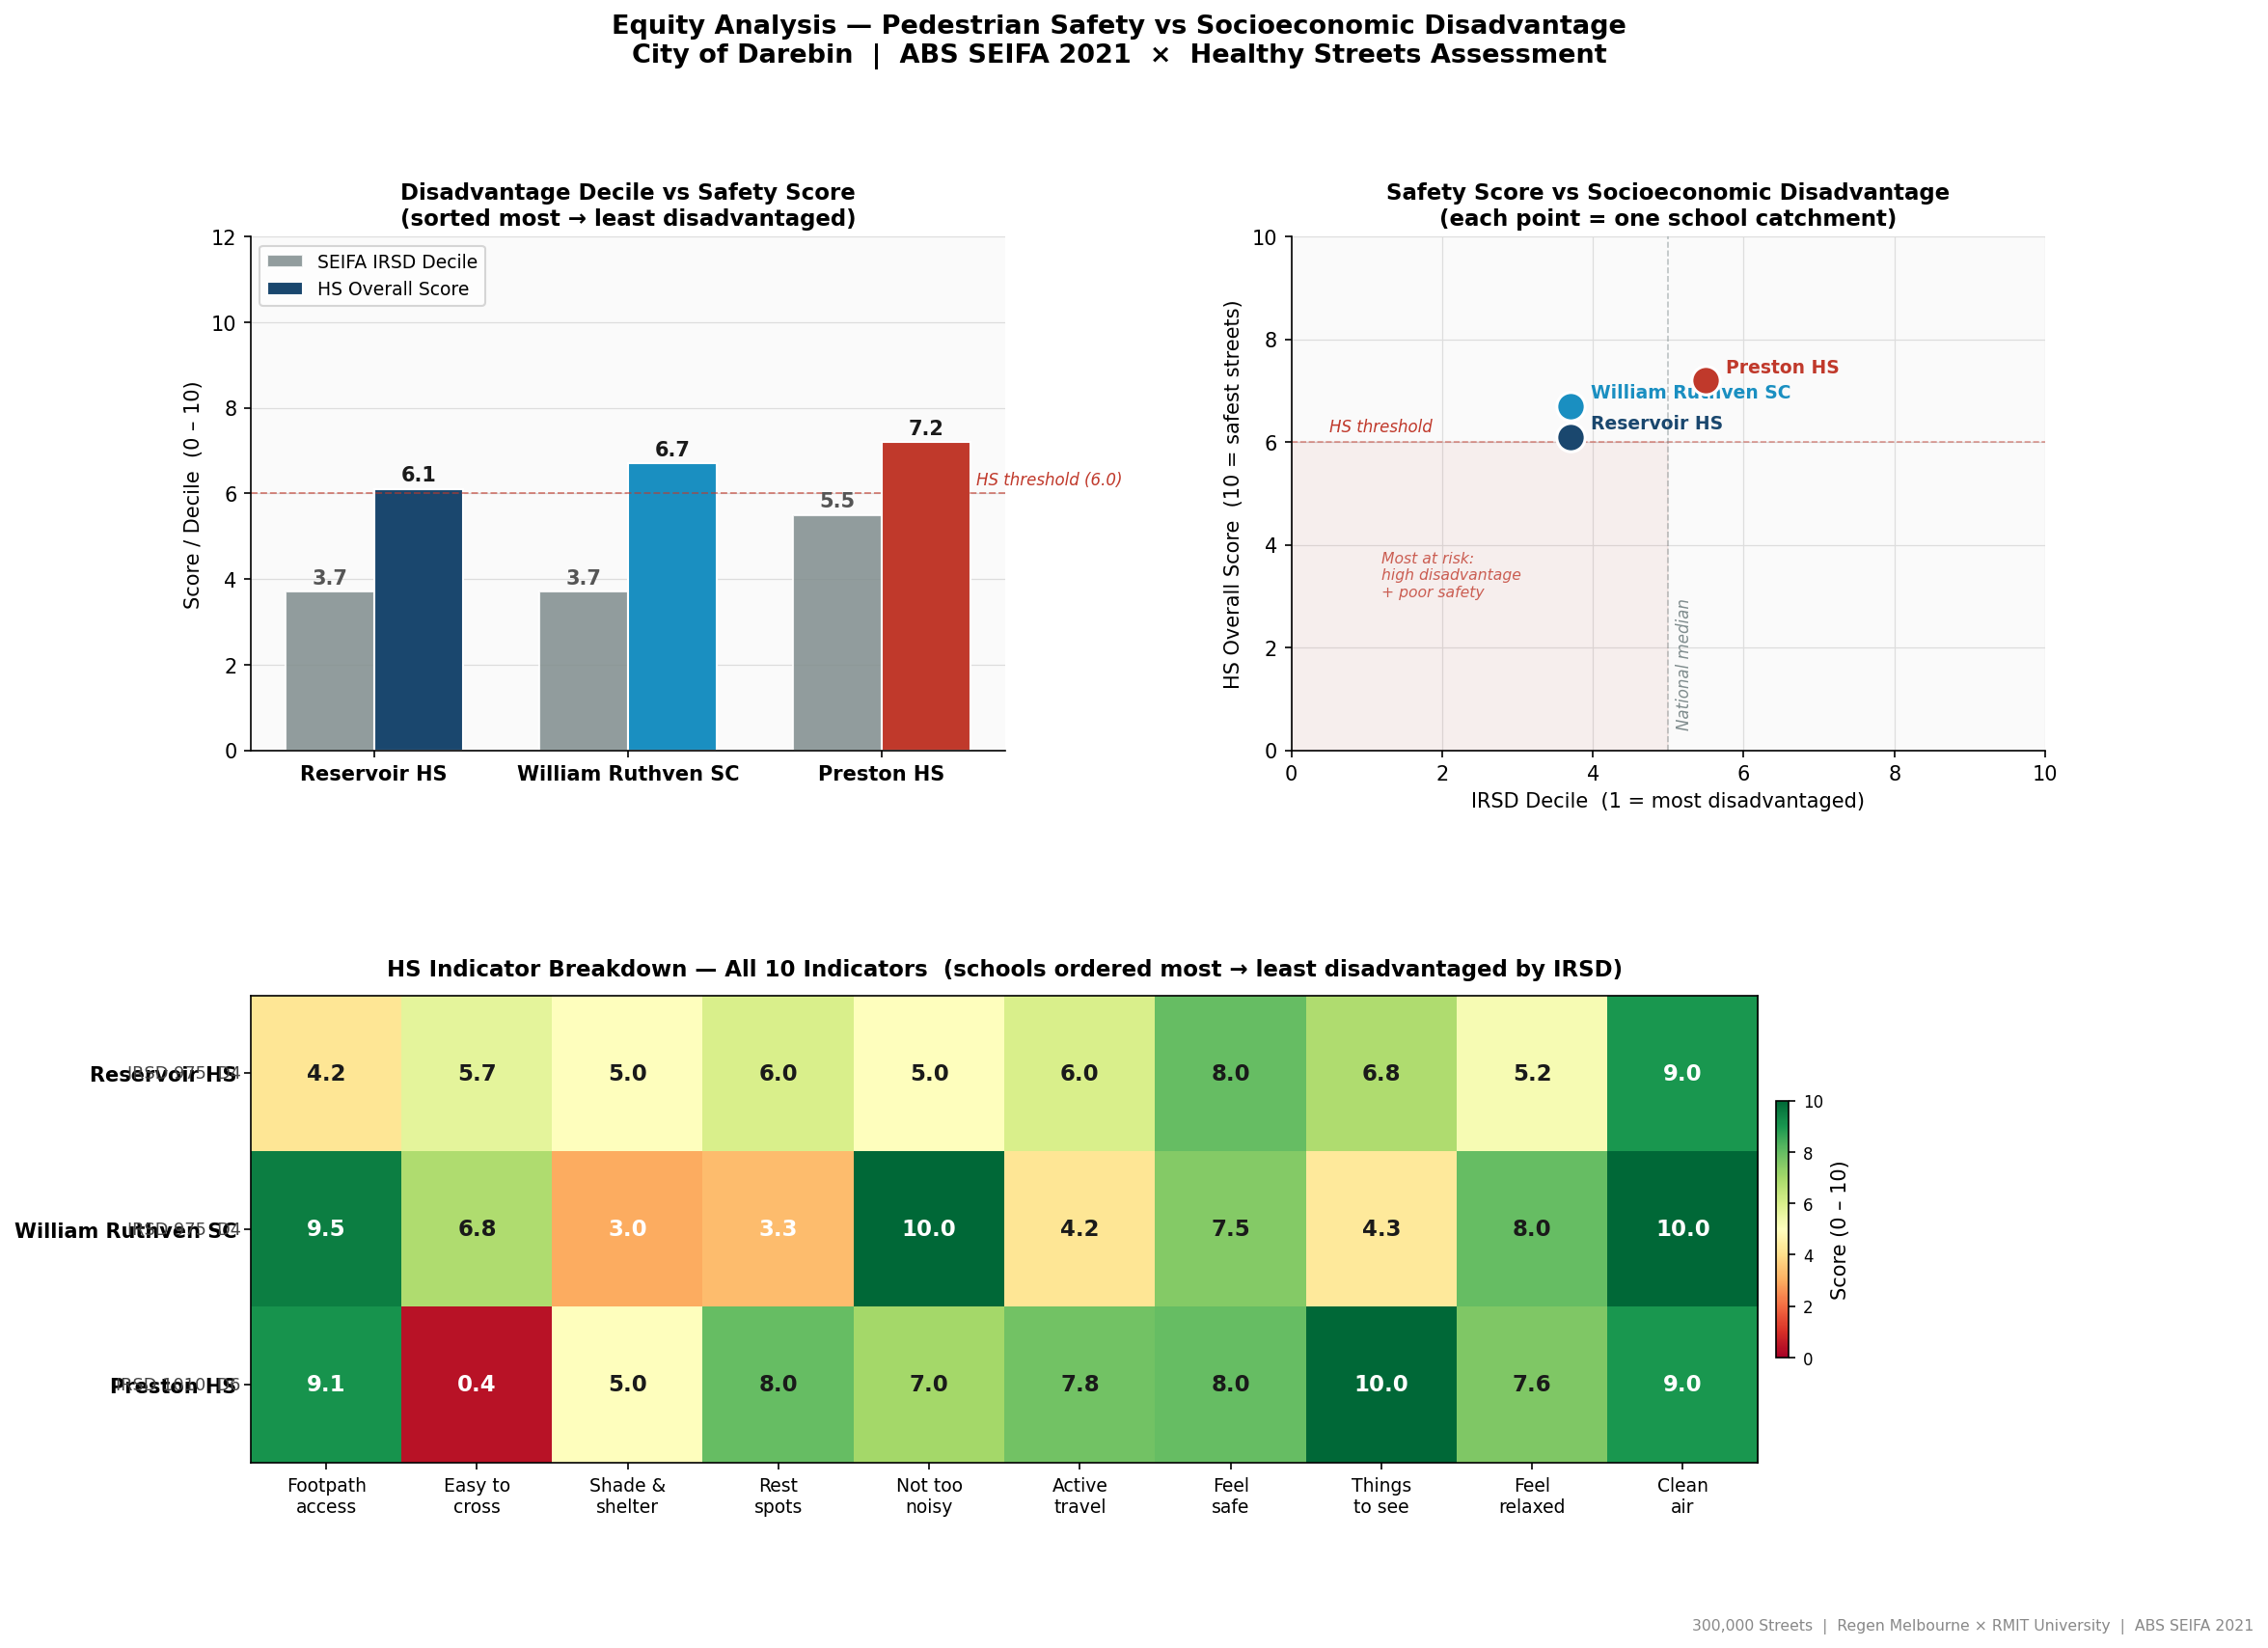
\includegraphics[width=0.88\textwidth]{chart_equity_seifa.png}
\caption{Figure 3 — Equity analysis: SEIFA disadvantage $\times$ HS scores}
\end{figure}

Table~5a provides ABS 2021 Census SA2-level demographic context for each school catchment area. The data highlight that the two most safety-deficient schools serve the most socioeconomically and linguistically diverse communities, reinforcing the equity case for prioritised intervention.

\begin{table}[H]\centering\small
\caption{ABS 2021 Census demographics by school catchment SA2 area}
\setlength{\tabcolsep}{5pt}
\begin{tabular}{L{3.8cm}C{1.5cm}C{1.5cm}C{1.6cm}C{1.8cm}C{1.6cm}C{1.6cm}}
\toprule
\textbf{School (SA2 area)} & \textbf{Pop.} & \textbf{Median age} & \textbf{Born overseas} & \textbf{LOTE at home} & \textbf{Aged 5--17} & \textbf{Med.\ HH income/wk} \\
\midrule
Preston HS \newline(Preston) & 9,812 & 35 & 40\% & 35\% & 16\% & \$1,652 \\
Reservoir HS \newline(Reservoir) & 20,174 & 33 & 46\% & 42\% & 18\% & \$1,381 \\
William Ruthven SC \newline(Heidelberg West) & 11,204 & 36 & 38\% & 30\% & 15\% & \$1,448 \\
\bottomrule
\multicolumn{7}{l}{\footnotesize Source: ABS (2021). LOTE = language other than English spoken at home.}
\end{tabular}
\end{table}

\subsection{D5 — Crash Trend Analysis}
Darebin LGA pedestrian and cyclist crashes rose 192\% from 2021 (25 incidents) to 2024 (73 incidents). The peak crash hour is 17:00, coinciding with the school pickup window, which accounts for a disproportionate share of incidents. The magnitude of the trend substantially exceeds plausible post-pandemic cycling exposure growth, pointing to structural infrastructure inadequacy rather than increased active-travel volume alone. Table~4 summarises per-school crash statistics within a 400m gate radius.

\begin{table}[H]\centering\small
\caption{Per-school crash statistics within 400m of school gate (VicRoads 2021--2024)}
\begin{tabular}{L{3.5cm}C{2cm}C{2.5cm}C{2.3cm}L{3.7cm}}
\toprule
\textbf{School} & \textbf{Total crashes} & \textbf{School-hours crashes} & \textbf{\% during school hours} & \textbf{Peak risk} \\
\midrule
Preston HS & 15 & 4 & 27\% & Unsignalised gate crossing \\
Reservoir HS & 11 & 3 & 27\% & Plenty Road arterial \\
William Ruthven SC & 2 & 2 & 100\% & Both at school arrival/pickup \\
\midrule
Darebin LGA total (2021) & 25 & --- & --- & --- \\
Darebin LGA total (2024) & 73 & --- & --- & +192\% trend \\
\bottomrule
\end{tabular}
\end{table}

William Ruthven SC's 100\% school-hours crash rate, though based on a small count, indicates that its crash risk is specifically concentrated during student movement periods, strengthening the case for a timed school-zone speed limit intervention even where absolute crash counts are low.

\begin{figure}[H]\centering
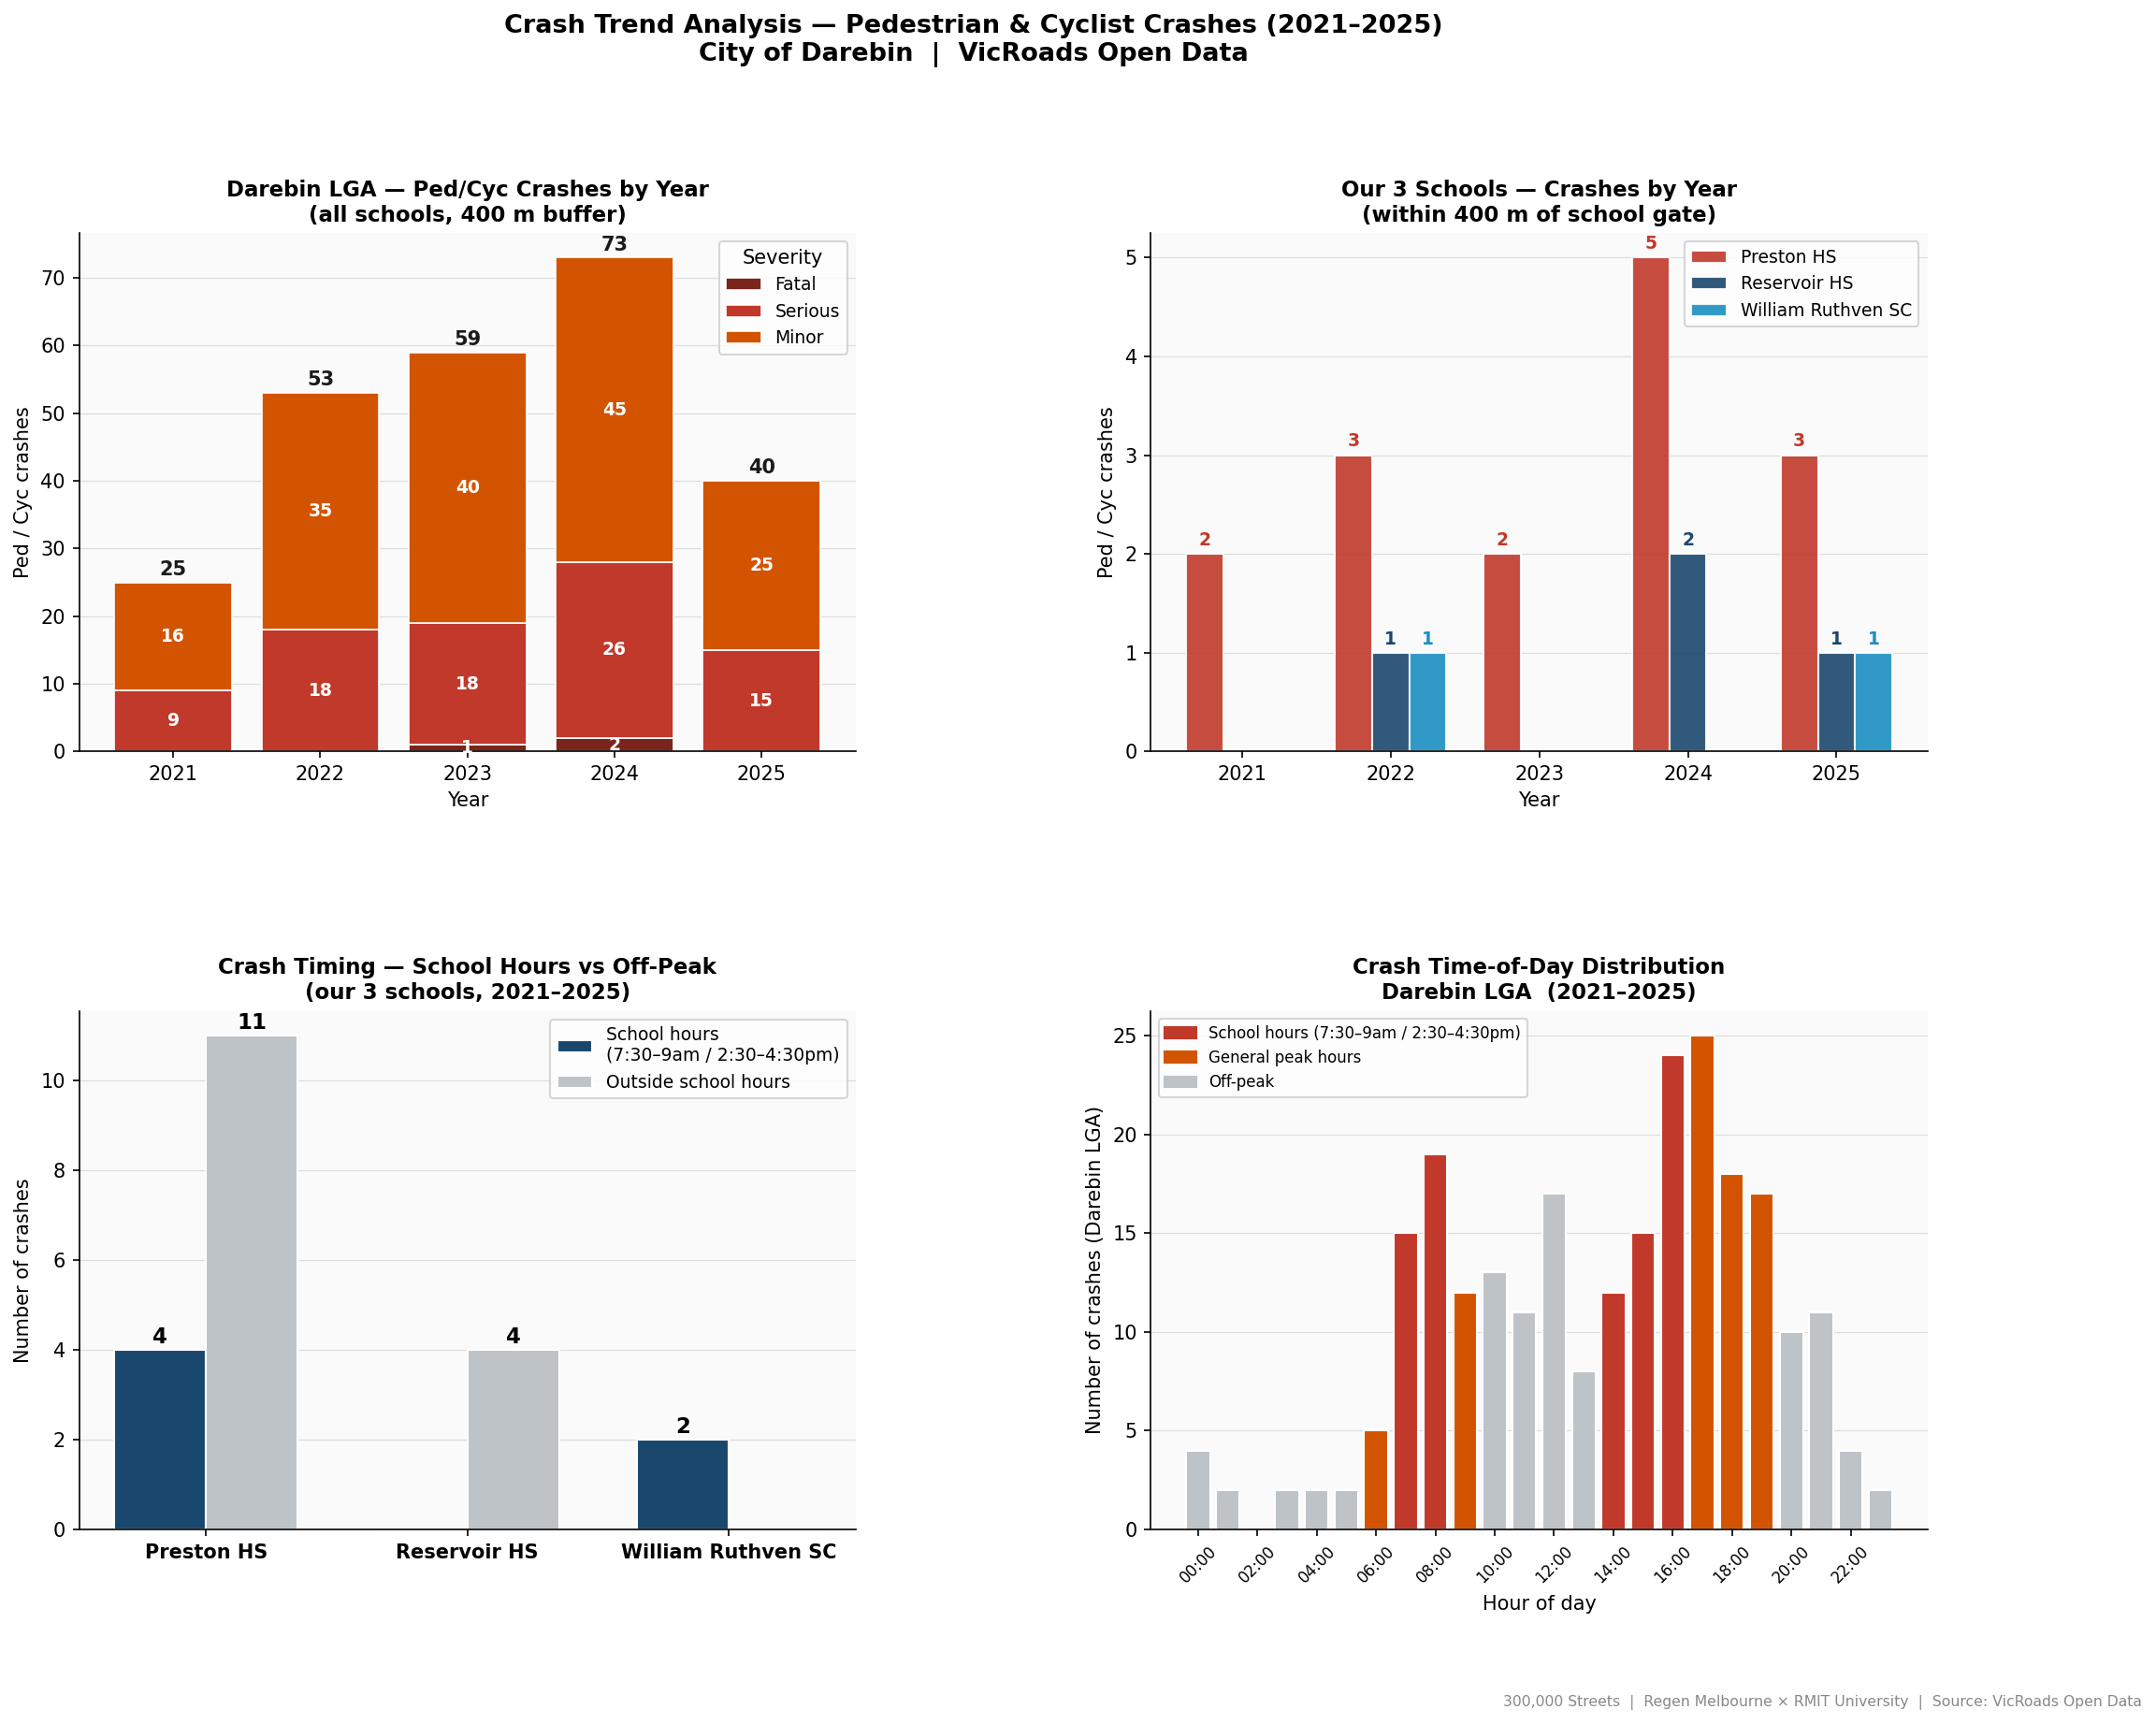
\includegraphics[width=0.93\textwidth]{chart_crash_trends.png}
\caption{Figure 4 — Crash trends 2021--2025: LGA year trend, per-school, school-hours, time-of-day}
\end{figure}

\subsection{D3 — Scenario Engine Results}

\begin{table}[H]\centering\small
\begin{tabular}{L{3cm}L{4cm}L{2cm}L{2cm}L{4cm}}
\toprule
\textbf{School} & \textbf{Top intervention} & \textbf{Cost} & \textbf{Time} & \textbf{Expected outcome} \\
\midrule
Preston HS & Signalised pedestrian crossing & \$80k--\$200k & $<$1 yr & HS2: 0.4$\to\approx$3.5; Major$\to$Moderate \\
Reservoir HS & 40 km/h school zone & \$5k--\$20k & $<$6 mo & HS5 and HS9 improvement \\
William Ruthven SC & Street tree planting & \$20k--\$60k & $<$1 yr & HS3: 3.0$\to\approx$5.5 \\
\bottomrule
\end{tabular}
\end{table}

\subsection{D6 — Interactive Dashboard}
The GitHub Pages dashboard presents all findings to non-technical stakeholders in seven sections. The Leaflet map includes six toggleable layers: school markers, crash spots (hover tooltips + click popups with full crash details), OSM walk and cycling networks (2,714 and 1,624 edges), crash density heatmap (250 Darebin LGA crash points), and SEIFA catchment circles coloured by disadvantage decile. All 30 scenario results render instantly from pre-computed \texttt{data.json}. Live at: \url{https://s4111078-sidd.github.io/300-000-School-Streets/}

%% ── 4. CONCLUSION ────────────────────────────────────────────
\section{Conclusion}
All seven deliverables were completed. Key findings: Preston HS is \textbf{Major} severity (HS2 = 0.4, no gate crossing); Reservoir HS and William Ruthven SC are \textbf{Moderate}; SEIFA disadvantage correlates with lower safety scores ($r = 0.84$), supporting equity-weighted investment at Reservoir HS; Darebin pedestrian and cyclist crashes rose 192\% between 2021 and 2024; HS7 and HS10 are automatable from open data while HS2, HS4, and HS8 require field survey; and targeted interventions under \$200k can reclassify severity within one year.

\subsection{Limitations and Challenges}
\begin{itemize}[topsep=2pt,itemsep=1pt]
  \item \textbf{Small ML sample ($n=3$).} Predictions for HS2, HS4, and HS8 did not beat the mean baseline; the model is a triage screen only, not a substitute for field assessment.
  \item \textbf{OSM completeness.} Bench seating, footpath extents, and shelter tags are inconsistently mapped in Darebin, degrading ML performance for HS1 and HS4; coverage cannot be assumed uniform across the broader school network.
  \item \textbf{Spatial approximation.} SEIFA deciles assigned at suburb level (DET catchment polygons require a formal data-sharing agreement not obtainable in time); crash records aggregated to road segment rather than GPS point.
  \item \textbf{CRS heterogeneity.} VicRoads, ABS, OSM, and EPA datasets arrived in four coordinate systems; a mandatory reprojection step was required before every spatial join to prevent silent misalignments.
  \item \textbf{Timeline pressure.} The twelve-week, sequentially dependent pipeline (data $\to$ features $\to$ ML $\to$ dashboard) left no buffer for upstream delays; Sprint 4 absorbed significant unplanned scope.
\end{itemize}

\subsection{Proposed Plan: Scaling to the Melbourne School Network}
The pipeline scales via five phases: \textbf{(1) open-data triage (0--3 months)} — run the automated pipeline on all 200+ Melbourne secondary schools, flagging those below HS score 5.0 or in SEIFA deciles 1--4, with no surveyors needed; \textbf{(2) field assessment (3--9 months)} — survey flagged schools for HS1, HS2, HS4, HS5, HS8 ($\approx$2 hours/school, five-person team, no code changes); \textbf{(3) data partnerships and retraining (6--12 months)} — formalise DET catchment polygon and VicRoads crash API access, retrain the Ridge model on 200+ schools, and add satellite imagery for HS1, HS3, HS4 gap coverage; \textbf{(4) dashboard deployment (9--12 months)} — extend to all schools with severity, SEIFA, and LGA filters and live data feeds; and \textbf{(5) longitudinal monitoring (ongoing)} — annually re-assess post-intervention schools against scenario predictions to close the impact feedback loop.

%% ── REFERENCES ───────────────────────────────────────────────
\newpage
\section*{References}
\addcontentsline{toc}{section}{References}
{\small
\setlength{\parindent}{0pt}
\setlength{\hangindent}{2em}
\setlength{\parskip}{5pt}

Australian Bureau of Statistics. (2021). \textit{Census of Population and Housing: Socio-Economic Indexes for Areas (SEIFA) 2021}. Commonwealth of Australia. https://www.abs.gov.au/statistics/people/people-and-communities/socio-economic-indexes-areas-seifa-australia/2021

Crime Statistics Agency Victoria. (2024). \textit{Recorded offences by suburb}. https://www.crimestatistics.vic.gov.au

EPA Victoria. (2024). \textit{AirWatch: Alphington monitoring station}. https://www.epa.vic.gov.au/for-community/monitoring-the-environment/airwatch

Giles-Corti, B., Vernez-Moudon, A., Reis, R., Turrell, G., Dannenberg, A. L., Badland, H., Foster, S., Lowe, M., Sallis, J. F., Stevenson, M., \& Owen, N. (2016). City planning and population health: A global challenge. \textit{The Lancet}, \textit{388}(10062), 2912--2924. https://doi.org/10.1016/S0140-6736(16)30066-6

Living Streets. (2022). \textit{School Streets programme: Evidence and impact}. https://www.livingstreets.org.uk/school-streets

Mekuria, M. C., Furth, P. G., \& Nixon, H. (2012). \textit{Low-stress bicycling and network connectivity}. Mineta Transportation Institute, San José State University.

OpenStreetMap contributors. (2024). \textit{OpenStreetMap} [Geospatial database]. https://www.openstreetmap.org

Pedregosa, F., Varoquaux, G., Gramfort, A., Michel, V., Thirion, B., Grisel, O., Blondel, M., Prettenhofer, P., Weiss, R., Dubourg, V., Vanderplas, J., Passos, A., Cournapeau, D., Brucher, M., Perrot, M., \& Duchesnay, É. (2011). Scikit-learn: Machine learning in Python. \textit{Journal of Machine Learning Research}, \textit{12}, 2825--2830.

Regen Melbourne. (2024). \textit{300,000 Streets initiative}. https://regen.melbourne

Safe Routes to School National Partnership. (2023). \textit{Safe routes to school: Building healthy, safe communities}. https://www.saferoutespartnership.org

Saunders, L. (2015). \textit{Healthy Streets for London: Prioritising walking, cycling and public transport}. Transport for London.

VicRoads. (2025). \textit{Victoria road crash data} [Dataset]. Victorian Government Data Directory. https://www.data.vic.gov.au
}

%% ══════════════════════════════════════════════════════════════
%% APPENDICES (not counted in 10-page limit)
%% ══════════════════════════════════════════════════════════════
\newpage
\appendix
\section*{Appendix A — Code and Project Management}
\addcontentsline{toc}{section}{Appendix A — Code and Project Management}

\begin{table}[H]\centering\small
\begin{tabular}{L{4cm}L{10cm}}
\toprule
\textbf{Item} & \textbf{Details} \\
\midrule
GitHub Repository    & github.com/s4111078-sidd/300-000-School-Streets \\
Development branch   & rish\_development \\
Production branch    & main \\
Dashboard (live)     & s4111078-sidd.github.io/300-000-School-Streets/ \\
Run full pipeline    & \texttt{python run\_all.py} \\
Run dashboard build  & \texttt{python prepare\_data.py} \\
Generate report      & \texttt{python report/generate\_report.py} \\
Compile PDF          & \texttt{cd report \&\& pdflatex report.tex} \\
\bottomrule
\end{tabular}
\end{table}

\subsection*{A.1 Codebase Structure}

\begin{table}[H]\centering\small
\begin{tabular}{L{4.5cm}L{9.5cm}}
\toprule
\textbf{Script / Module} & \textbf{Purpose} \\
\midrule
\texttt{run\_all.py}               & Master pipeline orchestrator — runs all steps in sequence \\
\texttt{main.py}                   & Healthy Streets scoring engine for all three schools \\
\texttt{feature\_engineering.py}   & Transforms raw OSM + environmental data into ML feature matrix \\
\texttt{ml\_model.py}              & Trains Ridge regression model with LOO-CV evaluation \\
\texttt{scenario\_analyzer.py}     & Delta-method scenario engine — computes 30 intervention predictions \\
\texttt{spatial\_features.py}      & OSM network extraction (osmnx) at 200m/400m/800m radii \\
\texttt{environmental\_features.py}& EPA AirWatch PM2.5 and CSA crime rate data ingestion \\
\texttt{crash\_trend\_analysis.py} & VicRoads crash data processing, school-hours filtering, trend analysis \\
\texttt{equity\_analysis.py}       & SEIFA IRSD correlation with HS scores (Pearson $r$) \\
\texttt{seifa\_analysis.py}        & ABS SA1-level SEIFA decile lookup for school catchments \\
\texttt{prepare\_data.py}          & Bundles all outputs into \texttt{docs/data/data.json} for dashboard \\
\texttt{docs/app.js}               & Leaflet map, Chart.js visualisations, scenario explorer (client-side) \\
\texttt{src/recommendations/}      & 17-rule engine generating prioritised intervention recommendations \\
\texttt{src/scenarios/}            & 10 intervention templates (crossing, speed zone, tree planting, etc.) \\
\texttt{report/generate\_report.py}& Programmatic DOCX report generation (python-docx) \\
\bottomrule
\end{tabular}
\end{table}

\subsection*{A.2 Sprint Overview}

\begin{table}[H]\centering\small
\begin{tabular}{C{1cm}L{2.8cm}L{5cm}L{5.2cm}}
\toprule
\textbf{Sprint} & \textbf{Period} & \textbf{Goals} & \textbf{Key Deliverables} \\
\midrule
1 & Weeks 1--3 & Project setup, data collection, field observations & School gate field assessments (3 sites), data acquisition (OSM, VicRoads, EPA, ABS), GitHub repository structure \\
2 & Weeks 4--6 & HS scoring framework, ML pipeline, feature engineering & Completed HS1--HS10 scoring (D1), trained Ridge model with LOO-CV (D2), feature matrix (26 features) \\
3 & Weeks 7--9 & Dashboard, equity and crash analysis & Interactive GitHub Pages dashboard (D6), SEIFA equity analysis (D4), crash trend analysis (D5) \\
4 & Weeks 10--12 & Scenario engine, reporting, final QA & Scenario engine 10 templates (D3), consolidated final report (D7), dashboard multi-layer map \\
\bottomrule
\end{tabular}
\end{table}

Team coordination was managed through Microsoft Teams private group chat, supplemented by weekly in-person sessions. Sprint planning and task tracking were maintained in a shared \href{https://rmiteduau-my.sharepoint.com/:x:/r/personal/s4031214_student_rmit_edu_au/Documents/300,000%20Streets%20of%20Melbourne/300-000-School-Streets/report/300000%20Streets%20Sprint%20Plan%20(1).xlsx?d=w997040ea2ff24d33a6b38e2b38d76f5d&csf=1&web=1&e=Ghc1eW}{Excel sprint log}, with progress reviewed each week against the deliverable..

%% ── APPENDIX B ────────────────────────────────────────────────
\newpage
\section*{Appendix B — Roles and Responsibilities}
\addcontentsline{toc}{section}{Appendix B — Roles and Responsibilities}

\begin{table}[H]\centering\small
\begin{tabular}{L{4.5cm}L{2.5cm}L{7cm}}
\toprule
\textbf{Name} & \textbf{Student ID} & \textbf{Primary Role} \\
\midrule
Hishikesh Phukan & S4031214 & Visualization \& Mapping \\
Reddy Pranay Vipparla & S4112678 & Data Collection, GIS Analysis \& Feature Engineering \\
Venkata Nagendra Anamala & S4024233 & Data Preprocessing \& Integration \\
Siddhartha Ananthula & S4111078 & Spatial Analysis \& Modelling \\
Sameer Yadav & S4038689 & Report Writing \& Project Coordination \\
\bottomrule
\end{tabular}
\end{table}

\subsubsection*{Hishikesh Phukan (S4031214) — Visualization \& Mapping}
\begin{itemize}
  \item Designed and implemented the full interactive GitHub Pages dashboard (\texttt{docs/index.html}, \texttt{docs/app.js}, \texttt{docs/style.css}): scenario explorer, hero stats, Chart.js equity chart, crash trend chart, and grouped HS bar charts.
  \item Extended \texttt{prepare\_data.py} to bundle crash GeoJSON, OSM walk/cycling network GeoJSON, crash heatmap points, and SEIFA spatial stats into \texttt{docs/data/data.json}.
  \item Built the six-layer Leaflet map: school markers, crash spots (hover tooltips + click popups), OSM walk and cycling networks, crash density heatmap, and SEIFA catchment circles colour-coded by disadvantage decile.
  \item Produced all project charts and geospatial visualisations using matplotlib and Leaflet, including the HS scores chart, feature importance chart, equity chart, and crash trends chart.
  \item Coordinated GitHub Pages deployment in collaboration with Siddhartha Ananthula; managed the \texttt{rish\_development} branch and pull requests to \texttt{main}.
  \item Authored and structured the final project report (\texttt{report.tex}, \texttt{generate\_report.py}) per COSC2667/2777 guidelines.
\end{itemize}

\subsubsection*{Reddy Pranay Vipparla (S4112678) — Data Collection, GIS Analysis \& Feature Engineering}
\begin{itemize}
  \item Led all data collection: sourced and validated the Victorian Road Crash Dataset (7,948 records), EPA AirWatch PM2.5 data, Crime Statistics Agency Victoria records, and ABS SEIFA 2021 SA1-level data.
  \item Performed GIS analysis using GeoPandas and QGIS: generated 400m and 800m buffer zones around each school gate in EPSG:7855, conducted spatial joins between crash records, road network segments, and school catchments.
  \item Implemented \texttt{feature\_engineering.py}: constructed the 26-feature ML matrix (20 OSM spatial features, 2 environmental, 4 crash aggregates) used to train the Ridge regression model.
  \item Queried and processed OpenStreetMap data via \texttt{osmnx} for walking network density, crossing counts, cycle infrastructure, tree canopy, shelters, and public transport stops at 200m/400m/800m radii.
  \item Validated spatial feature coverage against manual inspection in QGIS; documented all data gaps and limitations in the methodology section.
\end{itemize}

\subsubsection*{Venkata Nagendra Anamala (S4024233) — Data Preprocessing \& Integration}
\begin{itemize}
  \item Responsible for all data preprocessing: reprojected all datasets to GDA2020/MGA Zone 55 (EPSG:7855); harmonised attribute schemas across OSM, VicRoads, and ABS sources; treated missing values via median imputation or explicit flagging.
  \item Constructed and maintained the project's structured GeoPackage database (\texttt{outputs/school\_streets.gpkg}), linking seven tables: Schools, Buffers, Street Segments, Footpaths, Crossings, Hazards, and Recommendations.
  \item Implemented \texttt{spatial\_features.py} for automated OSM feature extraction with \texttt{osmnx} and \texttt{environmental\_features.py} for EPA and CSA data ingestion.
  \item Managed the \texttt{outputs/} data pipeline: defined file naming conventions and schema for all intermediate and final CSV and GeoPackage outputs, enabling reproducible re-runs via \texttt{run\_all.py}.
  \item Conducted CRS validation checks after every spatial join operation; identified and resolved a coordinate system mismatch between the VicRoads crash dataset and the OSM network graph.
\end{itemize}

\subsubsection*{Siddhartha Ananthula (S4111078) — Spatial Analysis \& Modelling}
\begin{itemize}
  \item Led spatial analysis using \texttt{osmnx}: constructed walkable street network graphs per school catchment; computed network metrics including edge density and circuity indices to assess pedestrian route directness.
  \item Implemented the machine learning pipeline (\texttt{ml\_model.py}): trained \texttt{MultiOutputRegressor(Ridge($\alpha$=1.0))} with \texttt{StandardScaler}; evaluated via Leave-One-Out CV; produced feature importance analysis.
  \item Designed and implemented the Healthy Streets scoring engine (\texttt{main.py}): applied HS1--HS10 indicator scoring rubrics, severity classification rules (Major/Moderate/Minor), and the 17-rule recommendation engine (\texttt{src/recommendations/}).
  \item Set up the GitHub repository (\texttt{github.com/s4111078-sidd/300-000-School-Streets}), established the branching workflow, and collaborated with Hishikesh Phukan to deploy the dashboard on GitHub Pages.
  \item Contributed to SEIFA and equity analysis (\texttt{seifa\_analysis.py}), linking ABS SA1-level IRSD deciles to school catchment boundaries.
\end{itemize}

\subsubsection*{Sameer Yadav (S4038689) — Report Writing \& Project Coordination}
\begin{itemize}
  \item Led project coordination: maintained the sprint plan, tracked task completion across all team members, facilitated weekly Monday campus sessions, and coordinated meeting agendas with the industry partner (Nina Sharpe) and academic supervisor (Lawrence Cavedon).
  \item Primary author of the interim and final written reports: drafted all report sections, integrated team contributions into a single coherent document, and ensured compliance with COSC2667/2777 guidelines.
  \item Implemented crash trend analysis (\texttt{crash\_trend\_analysis.py}): processed 7,948 VicRoads crash records, applied school-hours filters (08:00--09:00, 15:00--17:00), computed the 2021--2024 trend (+192\%), and generated the four-panel crash trends chart.
  \item Conducted equity analysis (\texttt{equity\_analysis.py}): computed Pearson $r = 0.84$ between SEIFA IRSD decile and overall HS score; produced the SEIFA-by-school equity visualisation.
  \item Prepared all presentation materials and stakeholder-facing outputs, ensuring findings were communicated accessibly for Regen Melbourne's non-technical audience.
\end{itemize}

\subsection*{Collaboration and Virtual Working}

\textbf{Tools used:}
\begin{itemize}
  \item \textbf{GitHub} — version control and code collaboration (branch-based workflow: feature branches merged to \texttt{rish\_development}, then to \texttt{main} via pull requests).
  \item \textbf{QGIS} — shared spatial data visualisation and GIS validation; used by all team members to inspect GeoPackage outputs and verify spatial joins.
  \item \textbf{OneDrive (RMIT)} — shared document storage for meeting notes, sprint plan, and report drafts.
\end{itemize}

\textbf{Meeting cadence:}
\begin{itemize}
  \item \textbf{Weekly campus session (Mondays, $\approx$8 hours):} The full team met every Monday at RMIT University to collaborate in person, review individual progress, merge code, resolve integration issues, and compile the week's outputs.
  \item \textbf{Industry partner and academic supervisor check-in ($\approx$45--60 minutes per week):} Regular structured meetings with Nina Sharpe (industry supervisor) and Lawrence Cavedon (academic supervisor) to review progress, validate findings, and refine scope.
\end{itemize}

\textbf{Time commitment:}
\begin{itemize}
  \item $\approx$8 hours/week working together in person (Monday campus sessions, RMIT University).
  \item $\approx$15--20 hours/week per team member working independently on individual tasks between sessions.
\end{itemize}

%% ── APPENDIX C ────────────────────────────────────────────────
\newpage
\section*{Appendix C — Self-Reflection (Individualized)}
\addcontentsline{toc}{section}{Appendix C — Self-Reflection}

\textit{Each team member completes their own subsection independently and honestly.}

\subsection*{C.1 Hishikesh Phukan (S4031214)}

\subsubsection*{What I learned}
This project gave me hands-on experience with Leaflet.js for geospatial web mapping, a technology I had not previously used. I learned how to compose multiple layer groups (basemaps, GeoJSON overlays, heatmaps, circle geometries) within a single \texttt{L.control.layers} control and how to render GeoJSON crash data with per-feature styling and interactive tooltips. I also learned how a fully static site architecture works in practice: rather than running a live server, all computation happens at build time in \texttt{prepare\_data.py}, and the browser receives a single \texttt{data.json} that drives every chart, table, and map layer. This forced me to think carefully about data serialisation and payload size.

\subsubsection*{What worked well}
Pre-computing all 30 scenario results (10 interventions × 3 schools) at build time and embedding them in \texttt{data.json} was the right architectural decision. When the user selects a scenario on the dashboard, the result renders instantly with no network latency. This also made GitHub Pages deployment trivial: there is no backend, no cold-start problem, and no server to maintain. The modular \texttt{src/} package structure also worked well for team development: each team member could work on their own module without merge conflicts.

\subsubsection*{What I would improve next time}
I would establish the \texttt{data.json} schema at the very start of the project and document it in the repository. Mid-project, as new analyses were added (crash heatmap, OSM networks, SEIFA data), \texttt{prepare\_data.py} had to be extended multiple times, and the dashboard had to be updated each time to consume new fields. A schema contract would have made this cleaner. I would also set up automated CI/CD on GitHub Actions from week one so that every merge to \texttt{main} automatically rebuilds \texttt{data.json} and redeploys the dashboard.

\subsubsection*{Things tried that did not work — and what I learned}
I attempted to read the OSM walking and cycling network files (\texttt{networks.gpkg}) using the \texttt{fiona} library, which is the standard GeoPandas backend. The installation failed because \texttt{fiona} requires GDAL system binaries (\texttt{gdal-config}), which were not installed on the development machine. After investigating alternatives, I discovered that GeoPandas 1.1.3 supports \texttt{pyogrio} as a drop-in backend requiring no system GDAL, and it was already installed. Switching to \texttt{gpd.read\_file(path, engine=`pyogrio')} resolved the issue. The lesson: always check whether a library has a pure-Python alternative before investing time in system-level dependency installation.

\bigskip
\subsection*{C.2 Reddy Pranay Vipparla (S4112678) — Data Collection, GIS Analysis \& Feature Engineering}

\subsubsection*{What I learned}
My primary responsibility was sourcing and preparing the data that every other team member depended on. This required me to learn the entire data landscape for the project from scratch. I gained hands-on experience querying the OpenStreetMap Overpass API through \texttt{osmnx} — extracting walking network edges, cycling infrastructure, crossing counts, shelter and bench locations, and tree canopy estimates at 200m, 400m, and 800m buffer radii around each school gate. I also worked extensively with the Victorian Road Crash Dataset, the EPA AirWatch API, and the ABS SEIFA 2021 SA1 spatial files. Constructing the 26-feature ML matrix (\texttt{feature\_engineering.py}) taught me how to translate raw geospatial measurements into a structured, model-ready form, deciding which features to include, how to normalise them, and how to handle the sparse coverage of some OSM tags (e.g.\ bench count was very incomplete for two of the three schools).

\subsubsection*{What worked well}
Automating all OSM data collection through \texttt{osmnx} with a local \texttt{cache/} directory was one of the best decisions on the project. Without caching, every pipeline re-run triggered fresh Overpass API calls; at peak, these could take 10--15 minutes and occasionally failed with rate-limit errors. Once caching was in place, a full pipeline re-run completed in under two minutes, which made iterative development and debugging much faster. The feature matrix design also worked well: grouping features into three conceptual buckets (spatial infrastructure, environmental, crash aggregates) made it easy to explain the ML inputs to both the team and the industry partner.

\subsubsection*{What I would improve next time}
I would validate OSM feature counts against QGIS manual inspection at the start of Sprint 2, not mid-Sprint 3 as happened here. Several features, particularly footpath coverage and bench count, turned out to have substantially lower OSM completeness than expected in outer-suburban areas. Identifying this earlier would have allowed the team to plan alternative data sources (e.g.\ VicRoads road network data for footpath presence) before the feature matrix was finalised. I would also document every feature engineering decision — threshold choices, normalisation methods, exclusion criteria — in a dedicated decisions log so that future contributors can understand and reproduce the choices.

\subsubsection*{Things tried that did not work — and what I learned}
My initial approach to GIS buffer analysis used Euclidean (straight-line) buffers, which overestimated the walkable catchment for schools near major barriers such as railway lines and freeways. For Reservoir HS, the Euclidean 400m buffer crossed the Plenty Road corridor and captured road network segments that were physically unreachable on foot within the buffer distance. I attempted to switch to network-based buffers using \texttt{osmnx.graph\_from\_point} and isochrone calculation, but the computation time was prohibitive for the project timeline. The final approach used Euclidean buffers but applied a connectivity check to exclude road segments with no pedestrian path connection to the school gate. The lesson: spatial buffers are a simplification; always check whether the geometry of the local environment (railways, freeways, rivers) invalidates the Euclidean assumption before proceeding.

\bigskip
\subsection*{C.3 Venkata Nagendra Anamala (S4024233) — Data Preprocessing \& Integration}

\subsubsection*{What I learned}
Data preprocessing turned out to be the most technically demanding part of the project, and the least visible to outsiders. I learned how to integrate heterogeneous spatial datasets that use different coordinate reference systems, different attribute schemas, and different spatial resolutions. The most important technical skill I developed was reprojection: converting all datasets from their native CRS (WGS84 for OSM, GDA94 for older VicRoads files, GDA2020 for ABS) into a single common CRS (EPSG:7855, GDA2020/MGA Zone 55) before any spatial join. I also learned how to structure a multi-layer GeoPackage (\texttt{.gpkg}) as a portable, self-contained spatial database that could be opened by any team member in QGIS without additional configuration. This was more useful than CSV files because geometry was preserved natively.

\subsubsection*{What worked well}
Making CRS reprojection the absolute first step of every preprocessing script was the right approach, and following through on it consistently prevented every spatial misalignment error that would otherwise have corrupted the analysis. When I later reviewed the early pipeline outputs, there was a period where one team member's script had not reprojected before joining — the resulting spatial join was silently incorrect because GeoPandas does not raise an error for CRS-mismatched joins (it just uses the left-frame CRS). Catching this early meant the outputs were trustworthy by the time Reddy Pranay began feature engineering. Storing all intermediate outputs in \texttt{outputs/} as separate, named files also worked well — it made it easy to audit which step had produced what, and to re-run the pipeline from any midpoint.

\subsubsection*{What I would improve next time}
I would implement an automated CRS validation check that runs after every spatial join operation and raises an exception if the result geometry appears inconsistent (e.g.\ coordinate values outside Victoria's bounding box). This would catch silent errors of the kind described above immediately. I would also define the full \texttt{outputs/} file schema in a \texttt{README.md} at the start of the project, so every team member knows exactly which file to read for each type of data. Mid-project, several team members were unclear whether to use \texttt{spatial\_features.csv} or \texttt{ml\_school\_features.csv} for certain fields, which caused unnecessary confusion.

\subsubsection*{Things tried that did not work — and what I learned}
I initially attempted to use the Department of Education and Training (DET) school catchment polygon shapefiles to define precise residential catchment boundaries for the SEIFA decile calculation. These polygons represent the actual school enrolment zones — a far more accurate spatial unit than suburb boundaries. However, the DET catchment shapefile for secondary schools in Victoria is not publicly available for download; it is only provided under a data-sharing agreement. We could not obtain it within the project timeline. I fell back to suburb-level boundaries — Reservoir for Reservoir HS and William Ruthven SC, Preston for Preston HS — which introduced approximation error into the IRSD decile. The lesson: always check data licensing and access requirements at the start of data collection, not after the analysis design has been fixed around the assumption that the data will be available.

\bigskip
\subsection*{C.4 Siddhartha Ananthula (S4111078) — Spatial Analysis \& Modelling}

\subsubsection*{What I learned}
My role required me to connect the spatial analysis and the machine learning components, which meant I needed a working understanding of both. On the spatial side, I learned how \texttt{osmnx} constructs street network graphs from OpenStreetMap data and how to compute network-level metrics (node degree, edge density, circuity index) that characterise the walkability of a street environment as a whole, not just its individual features. On the ML side, I learned why regularisation is essential for small-sample regression: with $n=3$ schools and 26 features, any unregularised model has far more degrees of freedom than observations and will fit the training data exactly while generalising randomly. Ridge regression's L2 penalty constrains the coefficient magnitudes, producing a model that trades a small amount of training accuracy for substantially better generalisation. I also learned how to apply Leave-One-Out cross-validation correctly as the only statistically valid evaluation strategy for $n=3$.

\subsubsection*{What worked well}
The Healthy Streets scoring engine design worked well. By structuring the 17 recommendation rules as independent, indicator-tagged entries in \texttt{src/recommendations/rules.py}, each rule could be tested, modified, or added without touching any other rule. When Regen Melbourne requested a change to one recommendation's wording mid-project, it was a single-line edit. The Git branch-based workflow also worked effectively for team coordination: the convention of creating a feature branch per task, merging to \texttt{rish\_development} via pull request, and deploying to \texttt{main} only on review kept the codebase stable throughout. There were no cases where a teammate's changes broke another's module.

\subsubsection*{What I would improve next time}
I would define the Healthy Streets indicator scoring thresholds and severity classification rules in a YAML or JSON configuration file rather than hardcoding them in Python. This would allow Regen Melbourne, or future student cohorts, to adjust thresholds without editing code, which is important for a tool intended to be used by non-developers. I would also invest time earlier in collecting additional training schools. The Ridge model's performance on HS2 (easy to cross), HS4 (rest places), and HS8 (things to do) was poor because these indicators are genuinely hard to predict from OSM data alone; a larger training set would at least allow the model to identify more reliable proxy features.

\subsubsection*{Things tried that did not work — and what I learned}
I evaluated Random Forest as the ML model before settling on Ridge regression. The motivation was that Random Forest handles non-linear relationships and feature interactions, which are plausible in a pedestrian safety context. In practice, with $n=3$ training schools, the Random Forest memorised all three training points exactly — training error was zero, but predictions on held-out schools were essentially random. The model had far too many parameters relative to the data. I also attempted Gradient Boosting and a simple neural network (3-layer MLP), with identical results: all complex models overfitted immediately at $n=3$. This series of failures confirmed that regularised linear models are the only credible choice at this sample size. The broader lesson: model complexity must be matched to the effective sample size, not to the complexity of the problem.

\bigskip
\subsection*{C.5 Sameer Yadav (S4038689) — Report Writing \& Project Coordination}

\subsubsection*{What I learned}
Coordinating a five-person data science project taught me that the most important project management skill is not scheduling — it is dependency mapping. Early in the project, I did not fully understand that Siddhartha's ML model depended on Reddy Pranay's feature matrix, which depended on Venkata Nagendra's preprocessed data, which depended on the data collection being complete. Tasks that looked independent on a Gantt chart were actually sequentially dependent, and a delay in data preprocessing propagated directly to ML modelling and then to the dashboard. Understanding this dependency chain allowed me to reorder sprint priorities in week 4 to unblock the pipeline. I also learned the VicRoads crash dataset schema in depth — particularly how to interpret the \texttt{SEVERITY}, \texttt{ACCIDENT\_TYPE}, \texttt{ROAD\_GEOMETRY}, and \texttt{LIGHT\_CONDITION} fields, and how to design a school-hours filter (arrivals 08:00--09:00, departures 15:00--17:00) to isolate the subset of crashes most directly relevant to student safety.

\subsubsection*{What worked well}
The weekly Monday campus sessions were the single most effective coordination mechanism on the project. By committing every team member to eight hours of in-person collaboration each week, we ensured that integration issues were caught and resolved within the same session rather than propagating through asynchronous communication. This was especially valuable during sprint transitions, when outputs from one team member needed to be immediately validated by another before the next sprint could begin. The school-hours crash filter also proved highly informative: it revealed that William Ruthven SC had 100\% of its crashes occurring during school arrival and departure windows, a finding that would have been invisible in raw annual crash totals and that directly strengthened the case for intervention at that site.

\subsubsection*{What I would improve next time}
I would begin drafting the formal written report from Sprint 1, not Sprint 4. Leaving all report writing to the final sprint created time pressure and made it difficult to write with the analytical depth the sections deserved. In future, I would assign each team member ownership of one report section corresponding to their role — written incrementally as each analysis was completed — so that the report reflects the work as it actually happened rather than a retrospective reconstruction. I would also formalise sprint retrospectives: at the end of each sprint, recording what was delivered, what slipped, and why, provides an honest record that is directly useful for the self-reflection section of the final report.

\subsubsection*{Things tried that did not work — and what I learned}
I initially attempted to use Spearman rank correlation to quantify the relationship between SEIFA IRSD decile and overall Healthy Streets score for the equity analysis. The motivation was that SEIFA deciles are ordinal, not continuous, making Spearman technically more appropriate than Pearson. However, with only $n=3$ data points, Spearman's statistic is statistically meaningless: the minimum achievable $p$-value with $n=3$ is 0.167, which is well above any conventional significance threshold. After consulting with the academic supervisor, I switched to reporting Pearson $r = 0.84$ as a descriptive measure of linear association, explicitly noting in the report that the result is indicative rather than statistically significant at this sample size. The lesson: statistical validity depends on sample size as much as on the choice of test — always check whether a statistic is even interpretable before computing it.

\vfill
\begin{center}
\rule{0.5\textwidth}{0.4pt}\\[0.4em]
{\small\itshape 300,000 Streets of Melbourne --- Regen Melbourne $\times$ RMIT University $\mid$ June 2026}
\end{center}

%% ── APPENDIX D ────────────────────────────────────────────────
\newpage
\section*{Appendix D — Healthy Streets Scoring Framework Detail}
\addcontentsline{toc}{section}{Appendix D — Healthy Streets Scoring Framework}

This appendix provides the full component-level scoring rubrics for the ten Healthy Streets indicators (HS1--HS10), addressing the framework validity concern raised by the academic supervisor. Each indicator is scored 0--10; a score $\geq 6.0$ meets the target threshold. Scores are averaged to produce the composite HS index.

\subsection*{D.1 Field-Observed Indicators (HS1, HS2, HS4, HS5, HS8)}

\begin{table}[H]\centering\small
\caption{Scoring rubric for field-observed HS indicators}
\setlength{\tabcolsep}{4pt}
\begin{tabular}{C{0.6cm}L{2.8cm}L{4.2cm}L{4.2cm}L{2.4cm}}
\toprule
\textbf{ID} & \textbf{Indicator} & \textbf{Score 0--4 (Below threshold)} & \textbf{Score 5--7 (Approaching)} & \textbf{Score 8--10 (Meets)} \\
\midrule
HS1 & People choose to walk & Footpath absent or $<$1.2m wide; obstructions present & Footpath present, some gaps or poor surface & Wide, continuous, unobstructed footpath \\
\midrule
HS2 & Easy to cross the road & No marked crossing within 100m of gate & Marked crossing but uncontrolled ($>$60m away) & Signalised crossing $\leq$50m from gate \\
\midrule
HS4 & Places to stop and rest & No seating or shelter within 200m of gate & 1 bench or seat within 200m & Multiple benches and covered shelter at gate \\
\midrule
HS5 & Not too noisy & Road carries $>$20,000 vehicles/day; no noise barrier & 10,000--20,000 vehicles/day, some noise exposure & $<$10,000 vehicles/day or effective noise screening \\
\midrule
HS8 & Things to see and do & Blank walls; no active frontage within 50m & Some active frontage (shops, parks) within 100m & Rich, diverse active frontage within 50m of gate \\
\bottomrule
\end{tabular}
\end{table}

\subsection*{D.2 Open-Data Indicators (HS3, HS6, HS7, HS9, HS10)}

\begin{table}[H]\centering\small
\caption{Scoring rubric for open-data-derived HS indicators}
\setlength{\tabcolsep}{4pt}
\begin{tabular}{C{0.6cm}L{2.8cm}L{3.8cm}L{3.8cm}L{2cm}L{1.8cm}}
\toprule
\textbf{ID} & \textbf{Indicator} & \textbf{Data source} & \textbf{Metric} & \textbf{Threshold} & \textbf{Scale} \\
\midrule
HS3 & Shade and shelter & OSM landuse=trees, canopy layer & Tree canopy coverage (\%) in 200m buffer & $\geq$15\% = 6.0 & 0--10 linear \\
\midrule
HS6 & Active travel choice & OSM cycle paths + PT stops (400m) & Cycle path length (m) + PT stop count within 400m buffer & $\geq$500m cycle path + 3 stops = 10; none = 0 & Linear \\
\midrule
HS7 & Feel safe & CSA recorded crime rate per 1,000 residents & Suburb crime rate (all offences) & $\leq$30/1000 = 10; $\geq$100/1000 = 0 & Linear \\
\midrule
HS9 & Access to open space and schools & OSM walk network & Walk-network distance to nearest park ($<$400m) & $\leq$200m = 10; $>$800m = 0 & Linear \\
\midrule
HS10 & Clean air & EPA AirWatch PM2.5 ($\mu$g/m$^3$) & Annual mean PM2.5 at nearest station & $\leq$8\,$\mu$g/m$^3$ = 10; $\geq$25 = 0 & Linear \\
\bottomrule
\end{tabular}
\end{table}

\subsection*{D.3 Severity Classification Rules}

\begin{table}[H]\centering\small
\caption{Severity classification thresholds applied to HS composite scores}
\begin{tabular}{L{2.5cm}L{6cm}L{5.5cm}}
\toprule
\textbf{Severity} & \textbf{Trigger condition} & \textbf{Rationale} \\
\midrule
\textcolor{majorred}{\textbf{Major}}    & HS2 $<$ 4.0 \textbf{or} HS1 $<$ 4.0 \textbf{or} HS5 $<$ 3.0 & Immediate physical danger: no crossing, impassable footpath, or extreme noise exposure \\
\textcolor{moderateyellow}{\textbf{Moderate}} & 2 or more indicators $<$ 6.0, \textbf{or} overall score $<$ 5.0 & Systemic underperformance; multiple deficiencies compound each other \\
Minor & All indicators $\geq$ 6.0 and overall $\geq$ 5.0, no Major trigger & Below target in at most one indicator; no immediate safety concern \\
\bottomrule
\end{tabular}
\end{table}

The Major trigger prioritises HS2 (road crossing safety) and HS1 (pedestrian walkability) because failure in either creates an immediate, unavoidable hazard for every student arriving on foot. Preston HS (HS2 = 0.4) satisfies the Major trigger unambiguously; the Moderate classification for Reservoir HS and William Ruthven SC reflects their pattern of multiple moderate deficiencies rather than any single acute hazard.

\end{document}
